\documentclass{newlayout}
%Bitte hier den enstprechenden Ort einsetzen z.B. Braunschweig und die Akademienummer
\Akademie{Braunschweig}{2015}{1}

\usepackage[ngerman]{babel}
\usepackage{misc}
\usepackage{multicol}
\usepackage[utf8]{inputenc}

%\usepackage{amsmath}%wird automatisch durch newlayout.cls geladen
\usepackage{amsfonts}

\usepackage{blindtext}

\usepackage{url}
\def\UrlBreaks{\do\a\do\b\do\c\do\d\do\e\do\f\do\g\do\h\do\i\do\j\do\k\do\l%
\do\m\do\n\do\o\do\p\do\q\do\r\do\s\do\t\do\u\do\v\do\w\do\x\do\y\do\z\do\0%
\do\1\do\2\do\3\do\4\do\5\do\6\do\7\do\8\do\9\do\-\do\_\do\/\do\%}
\urlstyle{same}

% hinzugefügt, um Fehler 'pdfTeX error (font expansion): auto expansion is only possible with scalable' zu vermeiden
\usepackage{lmodern}
\setkomafont{descriptionlabel}{\normalfont\bfseries}
\addtokomafont{paragraph}{\normalfont}
\usepackage{footnote}
\usepackage[flushmargin,hang,ragged]{footmisc}
\deffootnote{1em}{1em}{%
\textsuperscript{\thefootnotemark\ }
}
%\setlength{\abovedisplayskip}{5pt}
%\setlength{\belowdisplayskip}{5pt}


%%%%%Mathe-Definitionen
\newtheorem{Def}{Definition}
\newtheorem{Sat}{Satz}
\newtheorem{Bew}{Beweis}
\newtheorem{Thm}{Theorem}

\setlength\abovedisplayshortskip{0pt}
\setlength\belowdisplayshortskip{0pt}
\setlength\abovedisplayskip{3pt}
\setlength\belowdisplayskip{3pt}
%%%%Ende Mathe-Definitionen

\begin{document}

 %   \input{titel}
 \setcounter{page}{3}

\setcounter{tocdepth}{1}
 \tableofcontents

   \setcounter{secnumdepth}{1}


\setcounter{page}{7}
\setcounter{chapter}{0}

%Angabe, bis zu welcher Stufe die sections im Text nummeriert werden sollen.
      \settocdepth{2}



\course{1}{Learning from Data}%%% 
\begin{coursetitle}
  \centerline{Learning from Data} 
  \bigskip
  \Large \centerline{Mathematische Methoden des digitalen Zeitalters}
  \bigskip
 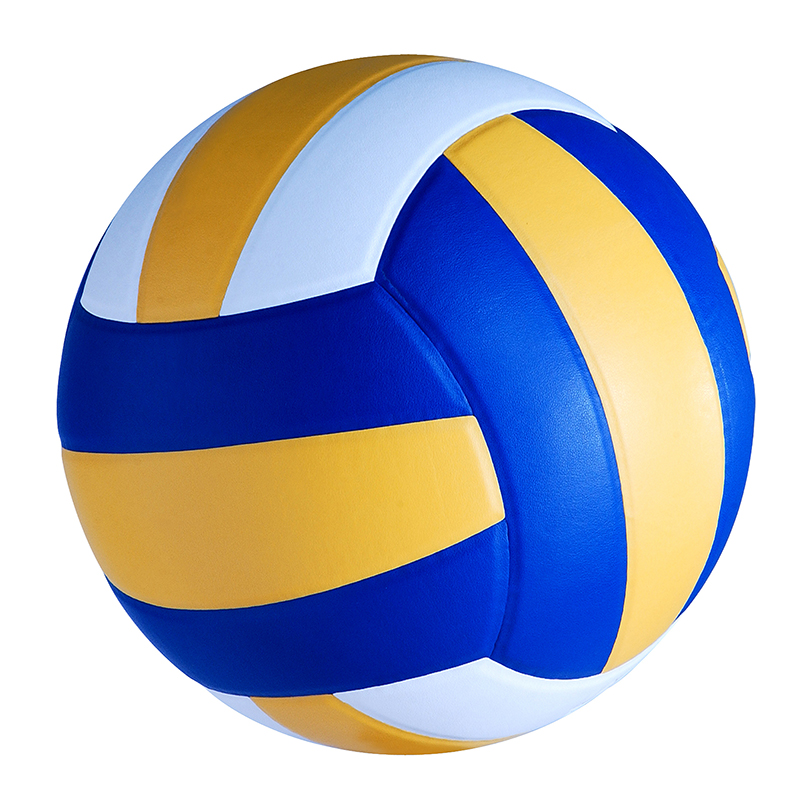
\includegraphics[width=.9\columnwidth]{Grafik-TempKursfoto.jpg}
 \label{fig:meinbild}
  \bigskip
\end{coursetitle}
%\begin{dsafigure}
%\begin{center}
%
\includegraphics[width=.9\columnwidth]{Titelbild-fehlt.png}
%\caption{meine Bildunterschrift}
%label{fig:meinbild}
%\end{center}
%\end{dsafigure}




\subsection{Konvexe Mengen}

\paragraph{Einführung}

Im Rahmen der Optimierung von konvexen Funktionen ist es erforderlich, den Begriff der konvexen Menge einzuführen. Um diese Thematik anschaulich darzustellen, verwenden wir zunächst verschiedene geometrische Figuren in Abbildung \ref{figure:Grafik-Optimierung_KonvexeMengen}, von denen einige konvex sowie andere wiederum nicht konvex sind. \\
Ist es eine direkte Verbindungsstrecke zwischen zwei beliebigen zu finden, die selbst ebenfalls in der Menge liegt, so ist die Menge konvex.

\begin{dsafigure}
\begin{center}
\includegraphics[width=0.4\textwidth]{\media Grafik-Optimierung_KonvexeMengen.pdf}
\label{figure:Grafik-Optimierung_KonvexeMengen}
\caption{Beispiele konvexer Mengen}
\end{center}
\end{dsafigure}

\begin{Def}[Konvexe Menge]

Eine Menge $X$ heißt konvex, falls für alle $x, y \in X$ und $\lambda \in \mathbb{R}$ und $\lambda \in [0,1]$ gilt:

\begin{equation}
\lambda x + (1 - \lambda) \in X
\end{equation}

\end{Def}

\subsection{Beispiele konvexer Mengen}

\paragraph{Kugel}

Ein Beispiel für eine konvexe Menge ist die Menge $S$ der Vektoren, die eine Kugel mit dem Radius $r = 1$, deren Mittelpunkt im Ursprung liegt, beschreibt:

\begin{equation*}
S = \{x \in \mathbb{R}^{n} | \lVert x \rVert \le 1\}
\end{equation*}

\paragraph{Quadrant}

Auch die Quadranten des kartesischen Koordinatensystems lassen sich durch eine konvexe Menge erfassen. So gilt z.~B. für den ersten Quadranten:

\begin{equation*}
L = \{ x \in \mathbb{R}^{n} | x_1 \ge 0, x_2 \ge 0, ..., x_n \ge 0\}
\end{equation*}

\paragraph{Eistüte}

Bei einer Eistüte bzw. einem quadratischen Kegel handelt es sich um ein weiteres Beispiel für eine konvexe Menge, da sie folgendermaßen für $x \in \mathbb{R}^{n-1}$ und $t \in \mathbb{R}$ beschrieben werden kann:

\begin{equation*}
Q = \{(x, t) \in \mathbb{R}^{n} | \lVert x\rVert ^{2} \le t\}
\end{equation*}

\paragraph{Box}

Die Menge von Vektoren in $B \subseteq \mathbb{R}$ bilden eine konvexe Menge in Form einer Box mit der Seitenlänge 2, deren Mittelpunkt im Ursprung liegt:

\begin{equation*}
B = \{x \in \mathbb{R}^{n} | |x_{i}| \le 1, i = 1, ..., n\}
\end{equation*}

\subsection{Konvexe Programme}

\paragraph{Einführung}

Bei einem konvexen Programm handelt es sich um die Optimierung einer Funktion $f$, die vom Parameter $x$ abhängig ist. Wir versuchen diese Funktion unter Berücksichtigung von Nebenbedingungen zu minimieren. Hierbei sind sowohl die Zielfunktion als auch die Menge der Punkte, die die Nebenbedingungen erfüllt, konvex.

\begin{Def}[Konvexes Programm]
Sei $f: \mathbb{R}^{n} \rightarrow \mathbb{R}$ eine konvexe Funktion und $X \subseteq \mathbb{R}^{n}$, so ist das konvexe Optimierungsproblem bzw. Programm die Minimierung der Funktion $f(x)$ unter der Nebenbedingung, sodass $x \in X$.
\end{Def}

\paragraph{Lineare Programme}

Lineare Programme lassen sich durch lineare Funktionen beschreiben, z.~B. $f(x) = \langle c, x \rangle$. Darüber hinaus sind eine lineare Abbildungsmatrix $A$, z.~B. $A = \begin{pmatrix}1 & 0 \\ 0 & 1 \end{pmatrix}$, sowie ein Vektor $b$ und ein weiterer Vektor $c$, z.~B. $c = \begin{pmatrix}1 \\ 0 \end{pmatrix}$, gegeben. $x$ ist dann zulässig, wenn $x \in X$ mit $X: Ax \le b$ bzw. $X = \{x \in \mathbb{R}^{n} | Ax \le b\}$ erfüllt ist. \\
Ein Beispiel für ein lineares Programm wäre:

\begin{equation*}
f(x) = \langle \begin{pmatrix}1 \\ 0 \end{pmatrix}, \begin{pmatrix}x_{1} \\ x_{2} \end{pmatrix} \rangle = x_{1}
\end{equation*}

Für die Nebenbedingungen gilt:

\begin{equation*}
\begin{pmatrix}1 & 0 \\ 0 & 1 \end{pmatrix}
\end{equation*}

Für den Wertebereich des linearen Programms folgt: $x_{1} \le 1$, $x_{2} \le 1$.

\paragraph{Quadratische Programme}

Im Vergleich zu einem linearen Programm weist z.~B. eine Kostenfunktion im quadratischen Programm eine quadratische Form auf. \\
Beispielsweise sei ein quadratisches Programm $f(x) = x^{T}Qx$ mit $Q = \begin{pmatrix}1 & 0 \\ 0 & 1 \end{pmatrix}$. $f$ gilt es nun unter der Bedingung $x \in X$ für $X: Ax \le b$ zu minmieren:

\begin{align*}
f(x) &= x^{T}Qx \\
&= \begin{pmatrix}x_{1}, x_{2}\end{pmatrix} \begin{pmatrix}1 & 0 \\ 0 & 1\end{pmatrix} \begin{pmatrix}x_{1} \\ x_{2}\end{pmatrix} \\
&= \begin{pmatrix}x_{1}, x_{2}\end{pmatrix} \begin{pmatrix}x_{1} \\ x_{2}\end{pmatrix} \\
&= x_{1}^{2} + x_{2}^{2}
\end{align*}

%\input{Kapitel-2-Kapitelüberschrift}
%\input{Kapitel-3-Kapitelüberschrift}
%usw.

%\nocite{*} % alle referenzen anzeigen, sogar wenn sie nicht im text zitiert sind
\bibliography{lit}{}
\bibliographystyle{plain}
\end{document}
